\section{Quantiles Sketch}
\label{sec:quantiles}


Given a stream $A$ of items from an ordered domain, for every
$0< \phi < 1$, $\phi$-quantile of $A$ is an item with rank 
$\lfloor \phi |A| \rfloor$, where the rank of item $i$ is the
number of elements in $A$ smaller than $i$.
An $\epsilon$-approximate ~$\phi$-quantile is an element
with rank between $ (\phi-\epsilon) |A|$ and $ (\phi +
\epsilon) |A|$.
For every stream $A$, error $\epsilon$, and probability $\delta$,
a quantiles sketch algorithm produces a summary of $A$, which
supports $\epsilon$-approximate ~$\phi$-quantile queries for
every $0< \phi < 1$ namely, returning an element with rank between $(\phi-\epsilon)n$ and  $(\phi+\epsilon)n$ with probability
at least $1 - \delta$.

\subsection{Overview}
As in the $\Theta$ sketch, there
is a tradeoff between the summaries' space cost and query accuracy,
which has been  studied in the past.
In this work we build on top of an algorithm presented
in~\cite{}, whose storage cost grows logarithmically with the
input stream size.
Given a stream $A$, the storage cost of the algorithm is
$k 2^{log(\lfloor |A|/k \rfloor)}$, where $k = O((1/\epsilon)
\sqrt{log(1/\epsilon \delta)}$.
The main idea is to 
\emph{merge} two sets, $S_1$ and $S_2$, consisting of $k$ items each, to a
single set $S$ of $k$ items.  This is done by first taking the sorted union of the sets, and  
then, with equal probability, retaining either the even or the odd
items in the sorted order. 
This process is called \emph{zip}.


The algorithm maintains $\lfloor log(|A|/k) \rfloor$ weighted
levels, where each level is an array of size $k$ that either contains $k$ ordered
items or is \emph{invalid} (see Figure~\ref{fig:quantilesMerge}).
The weight of level $i$ is $2^{i-1}$.
In addition, the algorithm uses a
\emph{bitPattern} variable that indicates which levels are valid,
and a \emph{base Buffer} of size $2k$, which is filled with items
from the stream.
Every time the baseBuffer is full, it is propagated (in place) to
the levels arrays in the following way:
First find using the bitPattern the first invalid level in
the levels array, 
call it the \emph{target} level. At the end of
the propagation this level becomes valid, while all the
level beneath it become invalid.
Next, sort and zip the base buffer (with equal probability,
pick either the even or the odd items in the sorted order) into
the target level.
Repeat the following process from level $i=1$ to the
last level that precedes the target level:
Mergesort level $i$ with what is currently stored in the target
level into the base buffer, and then zip the base buffer into the
target level.
Finally, update the bitPattern to indicate that the target
level is now valid while all the levels beneath it are not.

The weight of level $i+1$ is twice the weight of level
$i$ because it was zipped one more time, and thus it
``represents'' twice of the number of items ``represented'' in
level $i$.
This is important for quantiles accuracy.
In order to get a quantile we first have to build an
\emph{auxiliary} object that contains two arrays: 
(1) a sorted array of items, \emph{Iarr}, which 
contains all the items from all the valid levels, and (2) an
array of weights, called \emph{Warr}, that maps every item in
Iarr to its weight.
Then, to get the $\phi$-quantile, we %of a stream $A$
find the first index $ind$ in $Warr$ such that the
sum of all weights in $Warr$ till index $ind$ is $\lfloor \phi |A|
\rfloor$, and return $Iarr[ind]$. The algorithm is illustrated in
Figure~\ref{fig:quantilesMerge}.
%Since it is not the focus of our paper we omit the error analysis
%of the algorithm, and refer the interested reader to~\cite{} for
%the proof and more details.

\begin{figure}[tb]
    \centering
    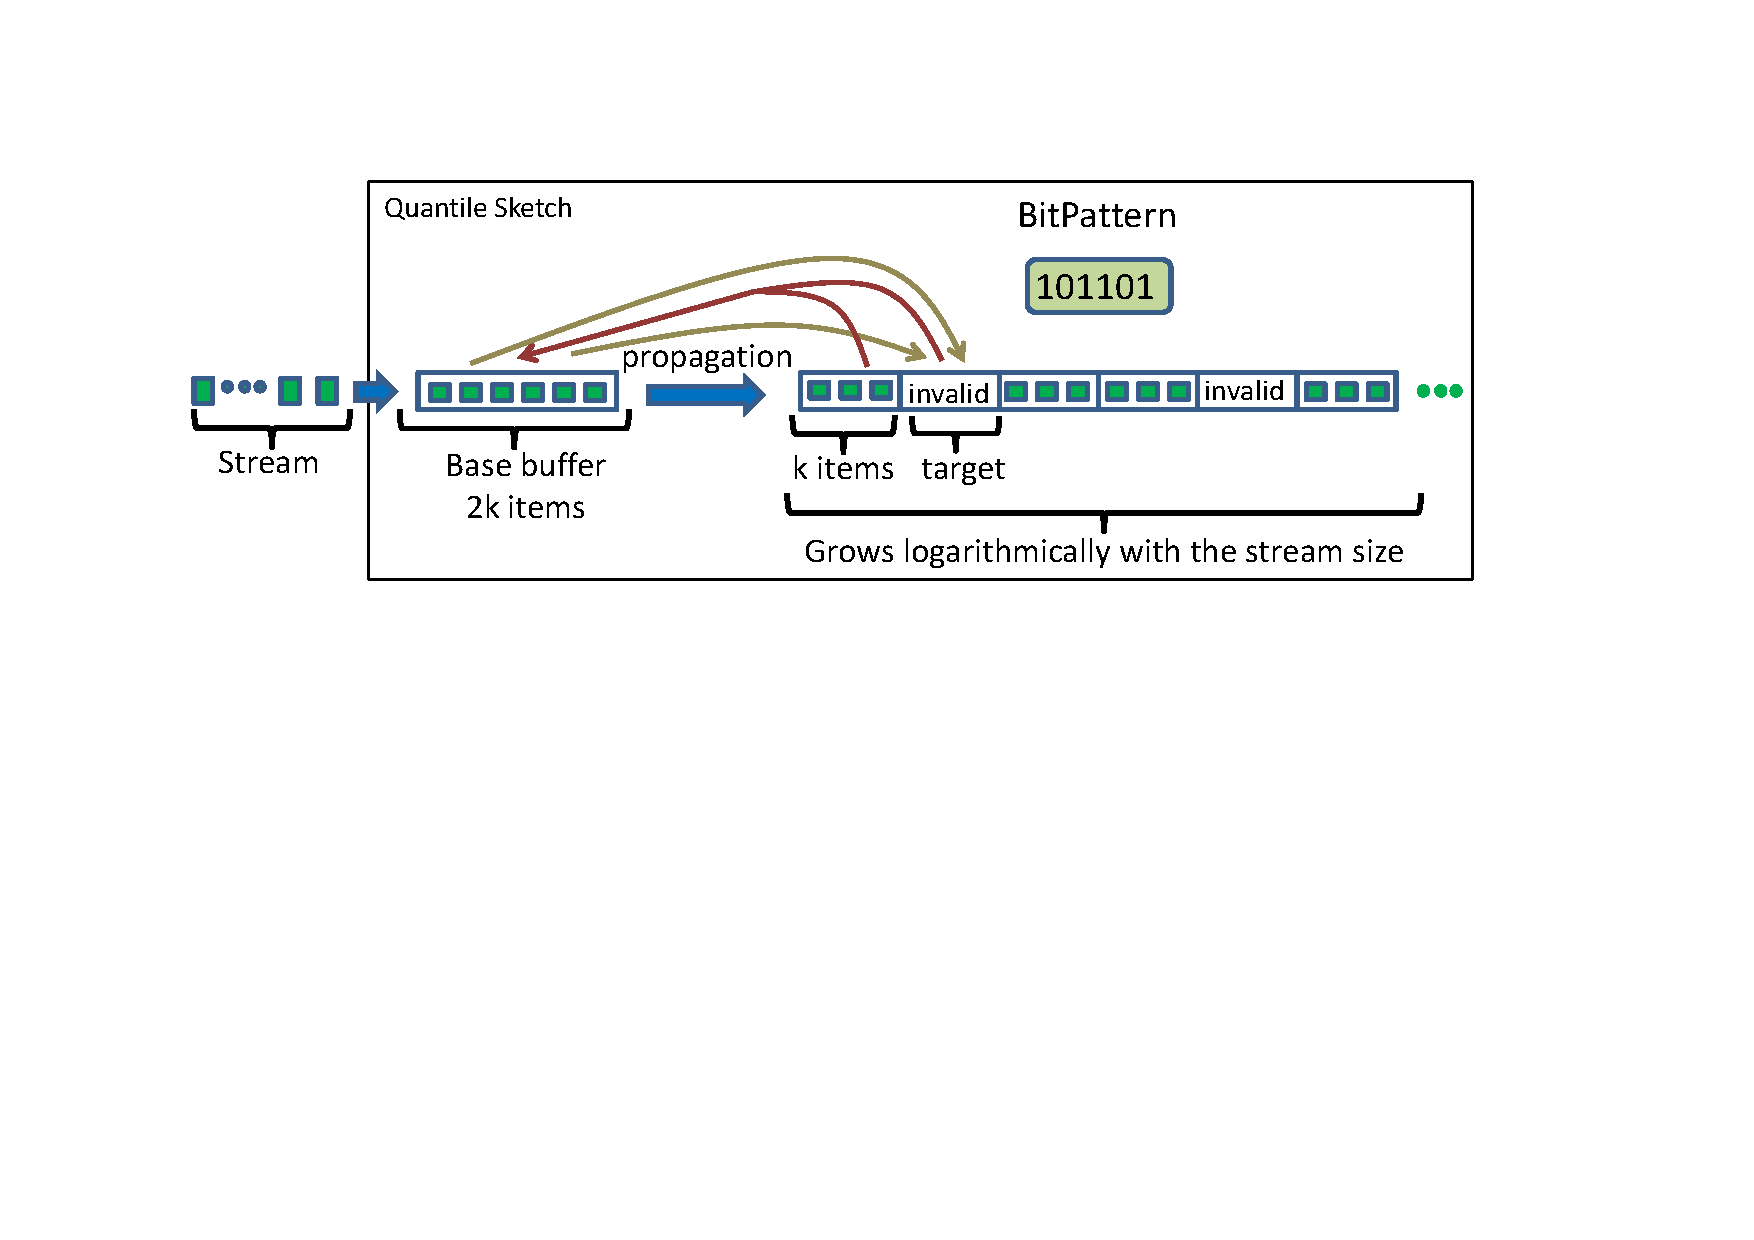
\includegraphics[width=3.2in]{images/quantilesPropogation.pdf}
    \caption{Quantile sketch: Propagating base buffer
    into the levels array.}
    \label{fig:quantilesMerge}
\end{figure}


\subsection{Concurrent Algorithm}

An efficient concurrent algorithm ought to allow  as much work as possible to be executed in parallel.
This is not an easy task since the propagation process (from the base buffer to the levels
array), which takes up most of the work in the algorithm, is
inherently sequential.
Our algorithm decreases the propagation rate without changing
the value of $K$: instead of propagating every $2K$ items we can
do it every $2^{L}K$, where $L \geq 0$ is a parameter that
impacts accuracy. Thus, we amortize the propagation cost and  increase
throughput.

The concurrent quantile algorithm exploits locality and minimizes
synchronization between a single propagation
background thread and many worker threads.
Every worker thread maintains a local sketch with bounded number
of levels; each level stores $b$ items. 
Every time the local sketch fills its last level, 
%and it is the only dataset 1M level 
the content of this  level is propagated to the
shared sketch via the background thread (See Algorithm~\ref{alg:concurrent-quantile}, and Figure~\ref{cocurrentQuntiles}).

\begin{algorithm*}[tb]
\small
\begin{multicols}{2}
\begin{algorithmic}[1]

%\State {\bf Sketch variables:}
\Vars
\State \emph{buf}, init $[ ]$ \Comment global samples
\State \emph{bitPattern}, init 0 \Comment global bit array of valid levels
\Statex
\ForEach{update thread $t_i$}
	\State \emph{q$_i$}, init empty \Comment local quantile sketch
	\State \emph{aux$_i$}, init $[ ]$ \Comment auxiliary array
	\State {\tt atomic} $P_i$, init $1$ \Comment for synchronization
\EndFor
\EndFor

\Statex
\Procedure{query}{$\phi$}
\State \emph{snapshot} $\leftarrow$ \emph{DoubleCollect(buf, bitPattern)}
\ForAll{valid \emph{lvl} in \emph{snapshot.bitPttern}} \label{l:caught-snapshot}
	\ForAll{\emph{sample} in \emph{snapshot.buf[lvl]}}
		\State append $\langle$\emph{sample},\emph{$2^{lvl}$}$\rangle$ to \emph{tuples}
	\EndFor
\EndFor
\State sort $tuples$ by $sample$
\State $pos \leftarrow \min {\{\lfloor N \times \phi \rfloor, N-1\}}$
\State $sum \leftarrow 0$
\State $ind \leftarrow 0$
\While{$sum \leq pos$}
	\State $sum \leftarrow sum + tuples[ind].weight$
	\State $ind \leftarrow ind + 1$
\EndWhile
\State \Return $tuples[ind-1].sample$ 
\EndProcedure
%\Statex

\Procedure{update$_i$}{$val$}
\State insert $val$ into $q_i$
\If{level $L$ in $q_i$ is the single valid full level }
		\State wait until $P_i>0$
		\State $aux_i \leftarrow$ level $L$ in $q_i$
		\State $P_i \leftarrow$ 0
		\State reset $q_i$
\EndIf
\EndProcedure

\Procedure{propagator}{}
\While {true}
\ForAll{update thread $t_i$ s.t. $P_i =0$}
		\State $tmpK \leftarrow aux_i$
		\State $P_i \leftarrow 1$
		\State \emph{target} $\leftarrow$ leftmost zero bit in \emph{bitPattern} $\leq L$
		\State \emph{bitPatternMask} $\leftarrow$ 0
		\For{$i \in \{L,\dots,target-1\}$}
				\State \emph{tmp2K} $\leftarrow$ mergeSort of \emph{tmpK} with \emph{buf[i]}
				\State \emph{tmpK} $\leftarrow$ zip \emph{tmp2K} \label{l:zip}
				\State set bit \emph{i} in \emph{bitPatternMask} to 1
		\EndFor
		\State \emph{buf[target]} $\leftarrow$ \emph{tmpk}
		\State set bit \emph{target} in \emph{bitPatternMask} to 1
		\State \emph{bitPattern} $\Leftarrow$ \emph{bitPattern} $\oplus$ \emph{bitPatternMask}
		\State $N \leftarrow N + K \times 2^{L}$
\EndFor
\EndWhile
\EndProcedure

\end{algorithmic}
\end{multicols}
\caption{Concurrent Quantile sketch algorithm. Maximum level in local sketches is $L$.}
\label{alg:concurrent-quantile}
\end{algorithm*}


The optimal number of local levels depends on the number of
concurrent worker threads.
Since  the propagation time is constant, more worker threads means each thread gets
less help from the background thread; we thus make sure that each thread needs help
less frequently by increasing the number of
local levels. 
%There is a balance point: too much levels means more delay in getting fresh results, not enough levels cause the propagation thread to become a bottleneck.

After triggering propagation to the shared sketch,
a worker thread starts filling its local sketch again.
As in the $\Theta$ sketch, the synchronization between the
propagation thread and  worker thread $t_i$ uses a 
single atomic variable $P_i$.

To propagate level $L$ from a local sketch to the shared sketch,
the propagation thread applies the mechanism of the
sequential quantiles sketch with the following
change:
Instead of starting from zipping the base buffer
into the target level, it starts from level $L$.
If level $L$ in the shared sketch is valid, the propagation
thread merges it (via merge sort) with the local level $L$ into
the base buffer, and continues the propagation to the next level
as before.
The target buffer in this case is the first invalid level that is
not smaller than $L$.
Otherwise, it simply copies the local level $L$ to the shared level
$L$.

Recall that in order to read (getQuantiles), readers build an
auxiliary object based on the levels array and the bitPattern
that describes it.
Therefore, to be able to read concurrently with
background propagation, a reader must obtain a \emph{snapshot} of the
levels array, which is achieved by obtaining 
 a successful  \emph{double collect}~\cite{snapshot}.
The bitPattern is an atomic variable so
that a propagation is visible to all readers after 
it is updated.
To get a snapshot, a reader repeatedly reads the bitPattern, then the levels array,
and then the bitPattern again.
If the bit pattern did not change between the two reads, the
reader has a consistent view.
Otherwise, it tries again.
In parallel, during the propagation process, the background
thread may read many levels, but write only to the target level,
which is invalid at this point.
Therefore, a reader can be sure that the valid levels it reads
between two identical reads of the bitPattern are consistent.
%even though the background thread is propagating in parallel.
%In addition, note that a reader do not have to read all valid
%levels each time it fails to obtain a successful double collect.
%Since a valid level may become invalid and then valid again
%(with different items) only after a higher invalid level becomes
%valid, if two sequential reads of the bitPatern has a
%common suffix, the reader must read only the valid levels in
%the different prefix of the later bitPattern read. 
%It is guaranteed that the valid levels in the suffix are unchanged.

The reads in this algorithm may suffer from starvation due to repeated changes of the bitPattern which prevent the readers from reading a consistent snapshot.
In practice, however, the propagation time (and thus
the time between bitPattern changes) is longer when the target
level is high.
%and every once in a while the background thread must propagate to a high level.
So, eventually the propagation is long enough for
a reader to obtain a snapshot of the levels array. 
The experiments we run show that the readers are 
much faster than the propagator, and the snapshot time is negligible relative to the time it takes to
build the auxiliary object.


\begin{figure}[tb]
    \centering
    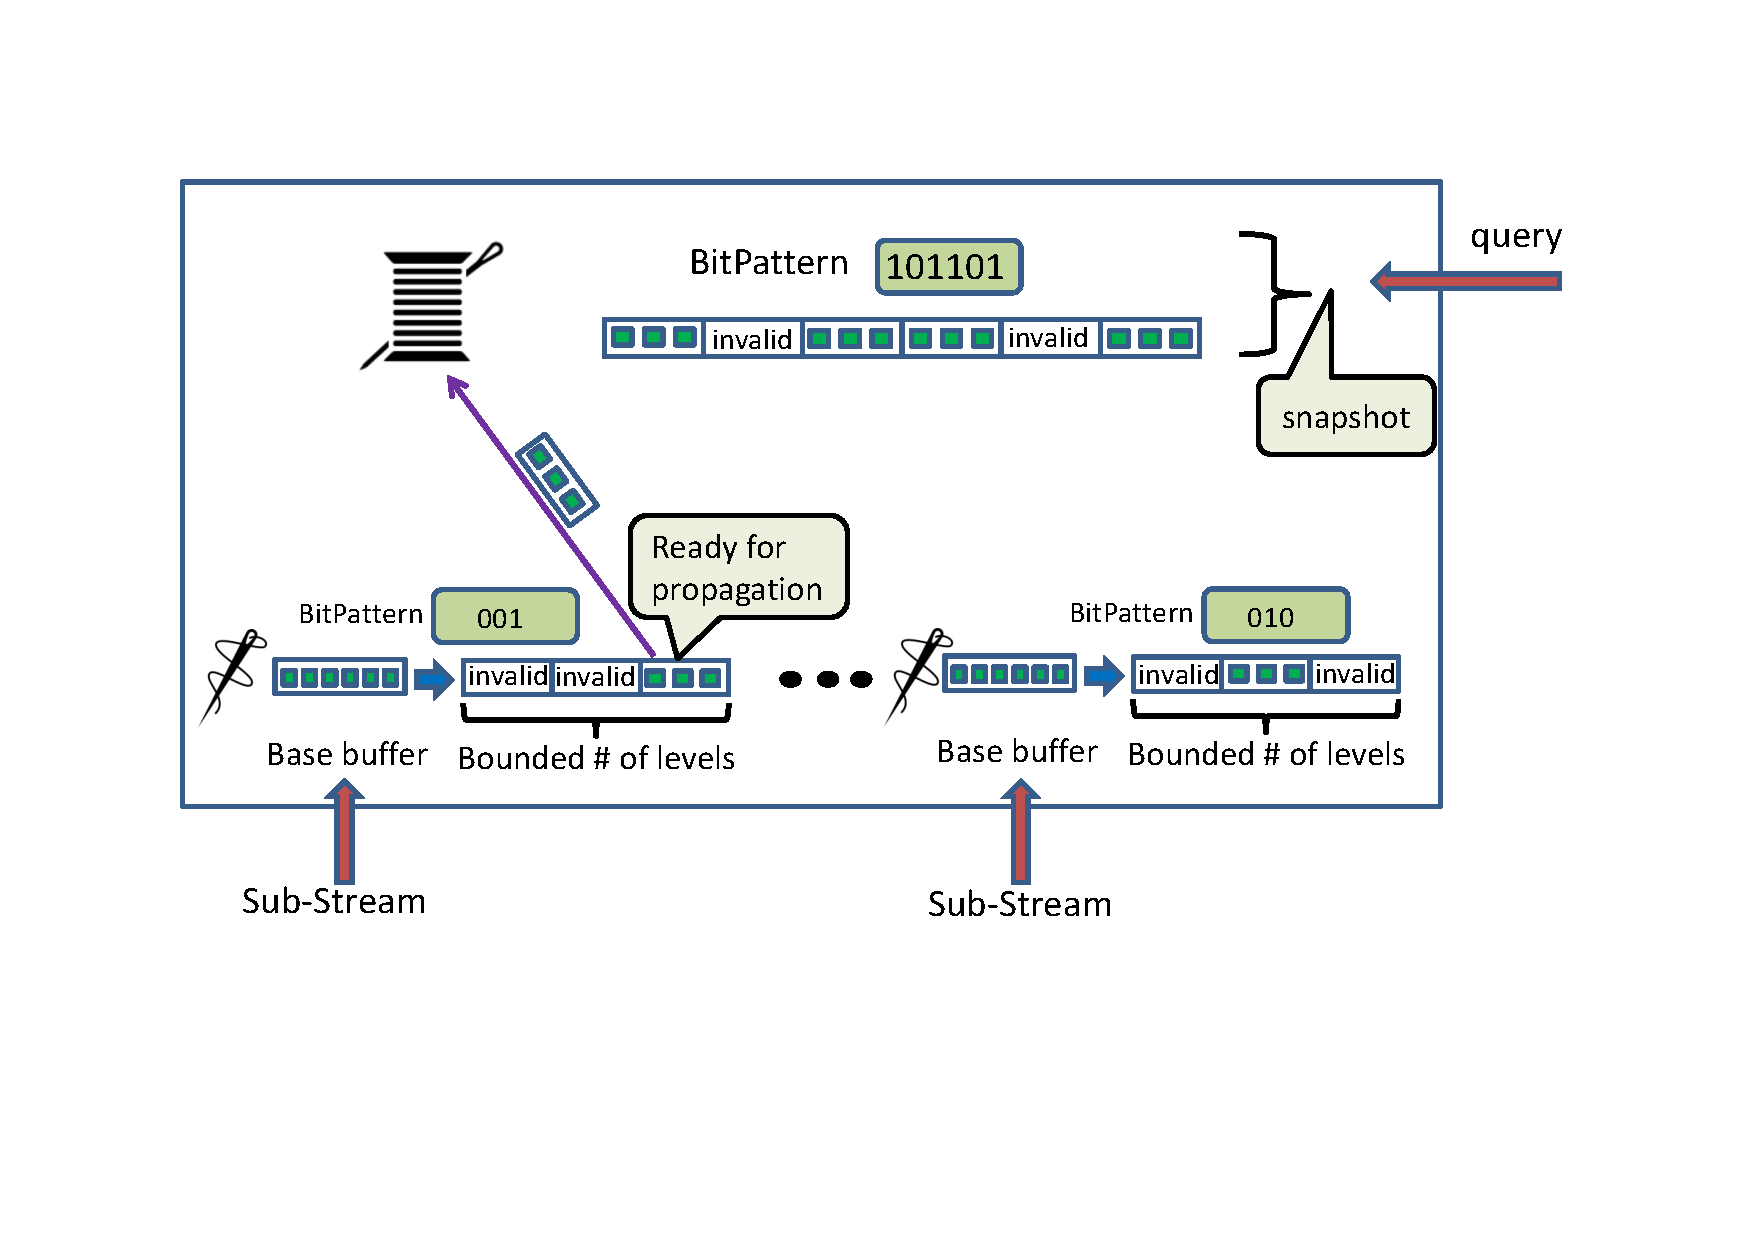
\includegraphics[width=3.5in]{images/cocurrentQuntiles.pdf}
    \caption{Concurrent Quantiles sketch architecture.}
    \label{cocurrentQuntiles}
\end{figure}

